%\documentclass[times]{MGS_class}

%\usepackage{wasysym}
%\usepackage{enumitem}
%\usepackage[T1]{fontenc}
%
%%-----
%%Title und Author angeben
%\title{GPU and CPU profiling\\ 
%of C++ and C\# programs}
%\author{Kernjak Martin \textsuperscript{1} and Kucher Josua \textsuperscript{2}}
%%die Institute weiter unten zu den zugehörigen superscripts angeben
%
%\begin{document}
%
%\twocolumn[{\csname @twocolumnfalse\endcsname
%\begin{center}
%\maketitle
%%\thispagestyle{empty}
%
%%------
%%ANGABE DER INSTITUTE ANFANG
%
%\noindent \scriptsize \textsuperscript{1}\textsl{FH Technikum Wien, Game Engineering und Simulation, Wien, AUT}\\
%
%%ANGABE DER INSTITUTE ENDE
%%------
%\end{center}
%%\normalsize
%\hspace{15mm}
%
%}]%---

\begin{abstract}
Profiling is a integral part of developing any performance critical programs. Various IDEs, Editors and other third party programs offer profilers. This paper introduces and evaluates the profilers of some of the industries biggest IDEs, Engines and Hardware Manufacturers.
\end{abstract}
\begin{keywords}
profiling, cup-profiling, gpu-profiling, gprof, unity engine, unreal engine 
\end{keywords}

\section{Introduction} \label{sec:Introduction}%ein Sternderl (engl. asterisk) \section*{Einleitung} unterdrückt die Nummerierung der Überschriften, dann werden sie in Adobe Reader aber auch nicht im Strukturbaum angezeigt

Profiling is an essential part of performance optimization in the development of software applications. In executable Programs, increases in speed of execution are very often desirable and profiling helps to achieve this especially if the implementation has routines that take up a large portion of the execution time. Finding these can help the programmer optimize these portions of code to achieve better performance and decrease the execution time significantly. \\
In most cases the software that needs to be optimized consists of a lot of small routines and a variety of abstraction levels. In some cases programs have been written by single individuals who comprehend all these abstractions but more often then not software is a group effort that evolved over time, this leads to shifting demands on abstraction levels. With the addition of external libraries which introduce additional abstraction levels into the program which are usually not examined further.\citep{graham_gprof:_1982}\\
 \cite{srivastava_atom:_2004} describe three kinds of program analysis tools, the first using program counters, the second kind are tracing data generation addresses and instructions and lastly simulators.
 The purpose of this work however is to give an introduction to various profilers and to show their functionalities so the inexperienced can use it as a guide to set up profiling in their project.
\section{Profiling} \label{sec:Introduction}

In essence profiling can be achieved in two different ways, execution counts and execution time, with both of them having respective benefits and problems.\\
Execution counts contain the exact amount of times a statement or routine is called. This can be useful when determining if the implemented algorithm is functioning correctly. In depth examination of such counters which are usually presented tabularily besides the source code, can help find error and overcomplexity in the program. In some ways this works similar to debugging as it helps to identify dead code. Execution counts ave a major downside though as they do not accurately represent the amount of time it took to execute a certain piece of code. This holds especially true if their are multiple abstraction levels.

\begin{lstlisting}[label={list:first},caption= Call Count example]
/*line Number---------------- count*/             
0001        if(x=foo)           0055
0002        functionX(foo)      0032
0003        if(x=baa) =         0055
0004        functionY(baa,foo)  0017
\end{lstlisting}

\fref{list:first} is an example of how call counts may be displayed inside code.

To determine execution times, two ways can be implemented. The first Method is sampling timestamps when entering and exiting a routine and calculating the time difference to gain the elapsed time. This become inherently complicated if the program uses time sharing due to the time slicing performed by the program. \cite{graham_gprof:_1982} describe another method as well which uses the sampling of the program counter at an arbitrary interval and use the distribution of these samples to determine the execution time of a program. Apparently this method works better for time sharing systems where the sampling interval can correspond with the time slicing of the program. Sampling also is independent of the operating system and only needs to be able to use interrupts. It is crucial that the sample intervals are uniform and are chosen sensibly. To high sample rates lead to problems in the profiled programs and to low sample rates are not accurately representing the time distribution. The difference between method one and two is their output, Method one can provide exact timings and method two is a statistical approximation.\citep{graham_gprof:_1982}

\section{ Evaluation and Instruction}


In the following sections various profilers will be discussed and introduced in a manner that will facilitate the understanding both in setup and usage of each profiler respectively. Furthermore multiple criteria (these are discussed at a later point) will be evaluated for each profiler to provide a fast way to asses usefulness for a specific project/use case. In this work only profilers used for C++ and C\# as well as game engineering related products, such as game engines are discussed, specifically the following:

\begin{enumerate}
    \item[-] Visual Studio Profiler
    \item[-] Unity Profiler
    \item[-] Unreal Profiler
    \item[-] Nvidia Nsight
    \item[-] AMD CodeXL
\end{enumerate}



\vfill\break
Criteria for the evaluation include the following and will be marked as \CheckedBox \text{ } if met by the respective profiler:

\begin{enumerate}
    \item CPU Sampling: The percentage of time spent in the function over the whole runtime of application.
        \begin{enumerate}
            \item[-] Call Counts: Number of Calls to a function over the whole program runtime.
            \item[-] Sampling Percentages: Sampling percentage of inclusive and exclusive percentages.
        \end{enumerate}
    \item Time Measurement: The actual time in seconds spent inside a function
        \begin{enumerate}
            \item[-] Function Level Measurement: Time Measurements of individual function in seconds.
            \item[-] Line Level Measurement: Time Measurements of individual lines in seconds.
        \end{enumerate}
    \item Memory Usage: Memory allocated and used by the application
        \begin{enumerate}[label*=\arabic*.]
            \item Memory Consumption: Combined stack and heap memory usage
                \begin{enumerate}
                    \item[-] Heap Allocation: Memory allocated on the heap.
                    \item[-] Stack Allocation: Memory allocated on the stack.
                \end{enumerate}
            \item Memory Allocation/Deallocation Time: Timestamps for memory allocation and deallocation.
        \end{enumerate}
    \item Multithread support: Profiling over multiple threads  
\end{enumerate}

\section{Visual Studio Profiler}

Visual Studio offers its own profiler. This profiler has been available in the professional version for some time but is now also available in the community edition since Visual Studio 2015.
It offers a simple real time statistic whenever the debugger is used. This shows the run-time, the used memory and the CPU utilization. The more in depth profiler can be used for multiple different profiling methods. These can then be analyzed in the performance explorer.\citep{microsoft_beginners_2015}

\subsection{Evaluation}

\begin{table}[htbp]
\begin{tabular}{p{5cm}|p{1cm}}
Criteria & Availability \\ \hline \hline
CPU Sampling & \CheckedBox \\ \hline
Call Counts & \CheckedBox \\ 
Sampling Percentages & \CheckedBox \\ \hline
Time Measurement & \CheckedBox \\ \hline
Function Level Measurement & \CheckedBox \\ 
Line Level Measurement & \CheckedBox \\ \hline
Memory Usage & \CheckedBox \\ \hline
Memory Consumption & \CheckedBox \\
Heap Allocation & \XBox \\ 
Stack Allocation & \XBox \\ 
Memory Allocation/Deallocation Time & \XBox \\ \hline
Multithread support & \CheckedBox \\ \hline
\end{tabular}
\caption{Results Visual Studio Profiler}
\label{tab:medfrequ}
\end{table}

The Visual Studio profiler supports almost every evaluated feature except for the exact Heap and Stack allocations. It only offers the current memory usage for a specific point in time, but does not show where in the code these allocations occurred.

\subsection{Profiling Methods}

The Performance Explorer offers 4 different profiling methods. 

\begin{enumerate}
    \item CPU Sampling 
    \item Instrumentation
    \item .Net memory allocation
    \item Resource Contention Data (concurrency)
\end{enumerate}

CPU sampling checks in which function the process currently resides in at regular intervals. The performance explorer can then be used to show the absolute and relative inclusive and exclusive sample count. This is a low overhead profiling method and is useful for an initial analysis.

Instrumentation is a more in depth profiling method that collects detailed timing data. As such the overhead is also considerably larger and can result in significant slow downs. Analyzing the profiling report is also much more time intensive.

The memory allocation profiling is only available in .Net and shows the functions which led to memory allocations and how many bytes were allocated.

Resource contention Data detects when one thread has to wait for another. More general data about how the threads are handled by the application is also collected. This lists the number of contentions and also how long they lasted.

These are the more in depth profiling methods but visual studio also offers CPU, GPU and memory tracking.

\citep{microsoft_how_2015} \citep{microsoft_understanding_2015}

\subsection{Starting a Profiling Session}

The solution should be loaded to start the profiling session. Go in the top menu to Debug->Start Diagnostics Tools Without Debugging.
A new window opens where the target and the profiling tool can be selected. The target defaults to the currently active solution but any project within the solution can also be selected among other targets.
Select $"$Performance Wizard$"$ and click start.
Another window will open where the profiling method can be selected. The concrete project can also be selected here.
Afterwards the program will be re-compiled and started. The profiling session ends when the main function finishes.
Finally a report will be generated from the profiling data.

The CPU, GPU and memory tracking tools work in a similar way but the user has to take explicit snapshots for the memory profiling.

\subsection{Using the Performance Explorer}

The performance explorer is automatically opened after a profiling session has finished.
Every Profiling session is listed on the left and the last report is opened automatically.
These reports can also be saved and loaded. The report section can be selected at the top under $"$Current View$"$.

The actual views are dependant upon the profiling method.

\subsection{CPU Sampling}

\begin{figure}[htbp]
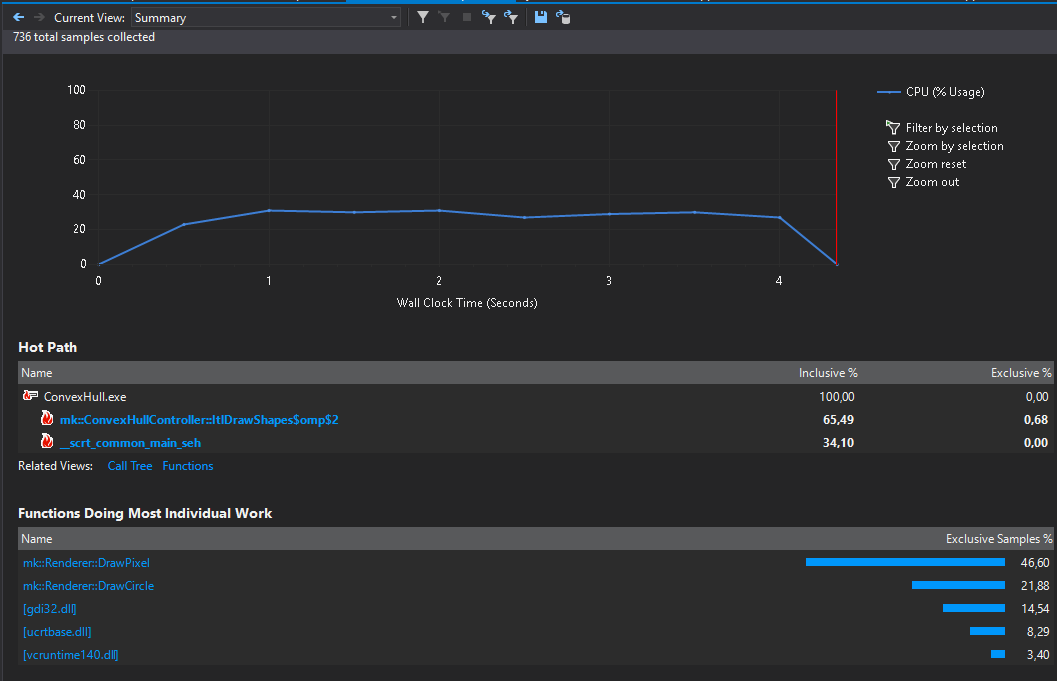
\includegraphics[scale = 0.28]{img/VisSummary.PNG}
\caption{Visual Studio Profiler CPU Sampling Report Summary}
\label{fig:VisualStudioProfilerSamplingSummary}
\end{figure}

This is the summary page. The graph at the top shows the CPU usage during the execution time.
Below is the $"$Hot Path$"$ which shows the branch of the call tree with the highest inclusive samples.
Below that are the functions with the highest amount of exclusive samples. Meaning that these function where covered by the most samples while disregarding samples in their child functions. Both of these offer a good starting point for optimization. The function can also be selected for a per function and line breakdown.

\begin{figure}[htbp]
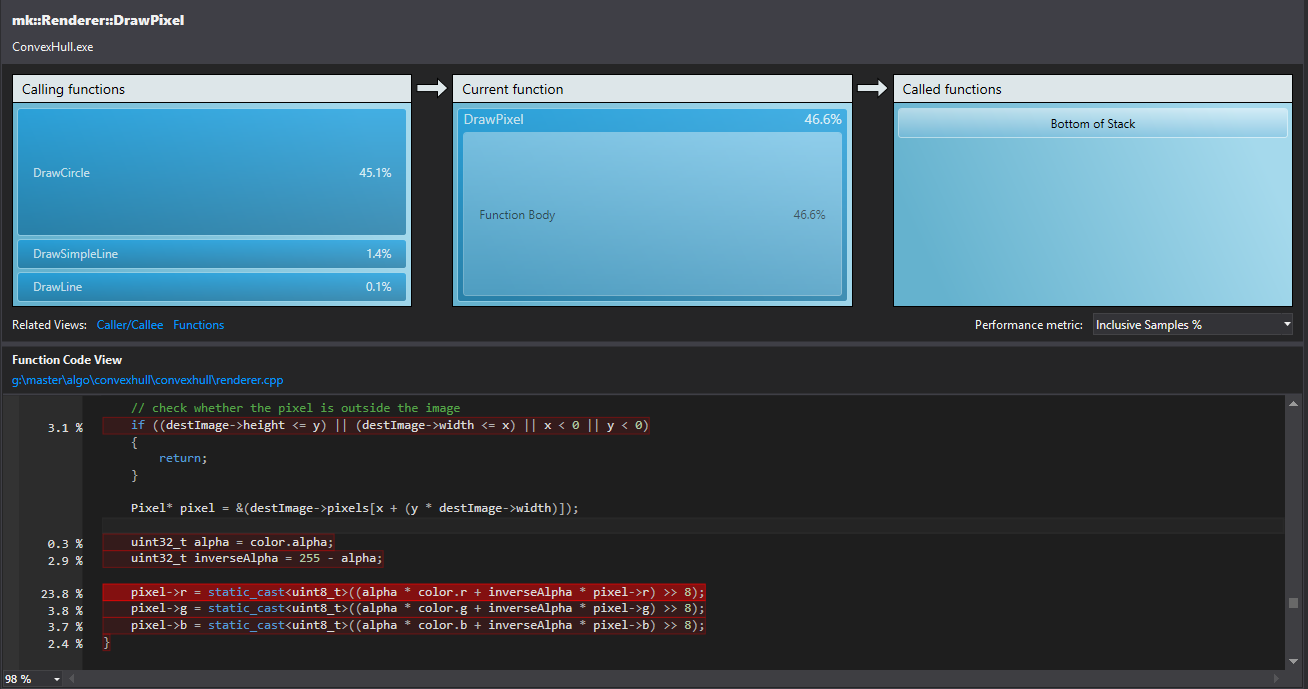
\includegraphics[scale = 0.225]{img/VisFunctionBreakdown.PNG}
\caption{Visual Studio Profiler CPU Sampling Function Breakdown}
\label{fig:VisualStudioProfilerSamplingFunctionBreakdown}
\end{figure}

The function breakdown shows the sample percentages for the caller functions and any function called by the current one.
The actual lines with the highest sample count are also highlighted below.

\begin{figure}[htbp]
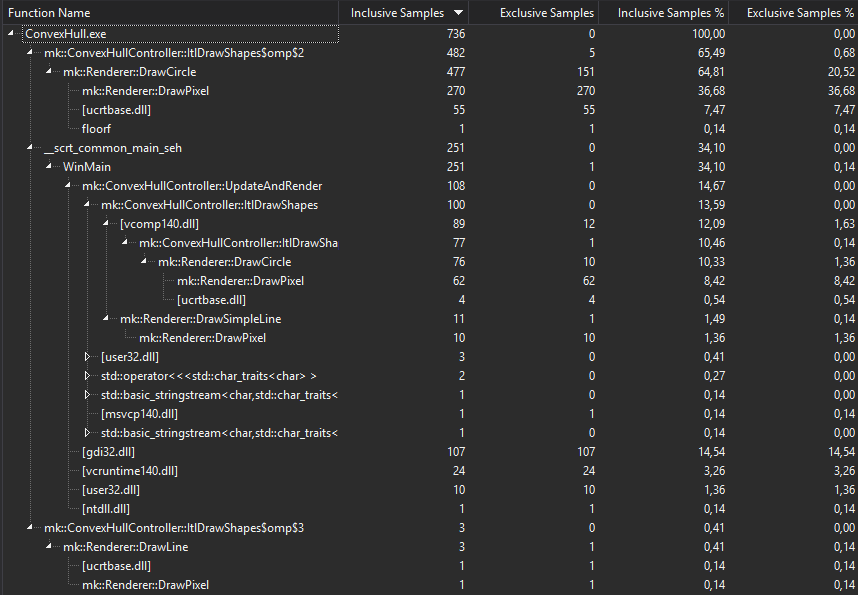
\includegraphics[scale = 0.34]{img/VisCallTree.PNG}
\caption{Visual Studio Profiler CPU Sampling Call Tree}
\label{fig:VisualStudioProfilerSamplingCallTree}
\end{figure}

There are also other views such as the aforementioned call tree.

\begin{figure}[htbp]
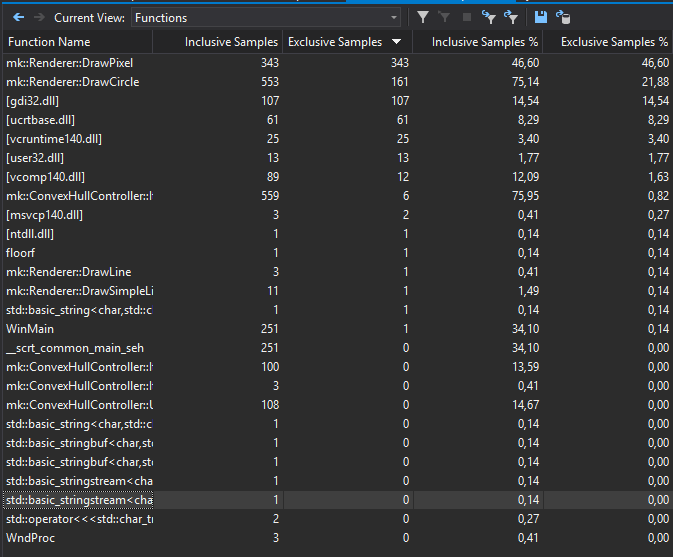
\includegraphics[scale = 0.42]{img/VisFunctions.PNG}
\caption{Visual Studio Profiler CPU Sampling Functions}
\label{fig:VisualStudioProfilerSamplingFunctions}
\end{figure}

And a complete function breakdown.

\subsection{Instrumentation}

The instrumentation report also includes real time measurements. The report structure is the same as for the CPU sampling but the
values are based on the actual execution time instead of the more in-precise samples.

\begin{figure}[htbp]
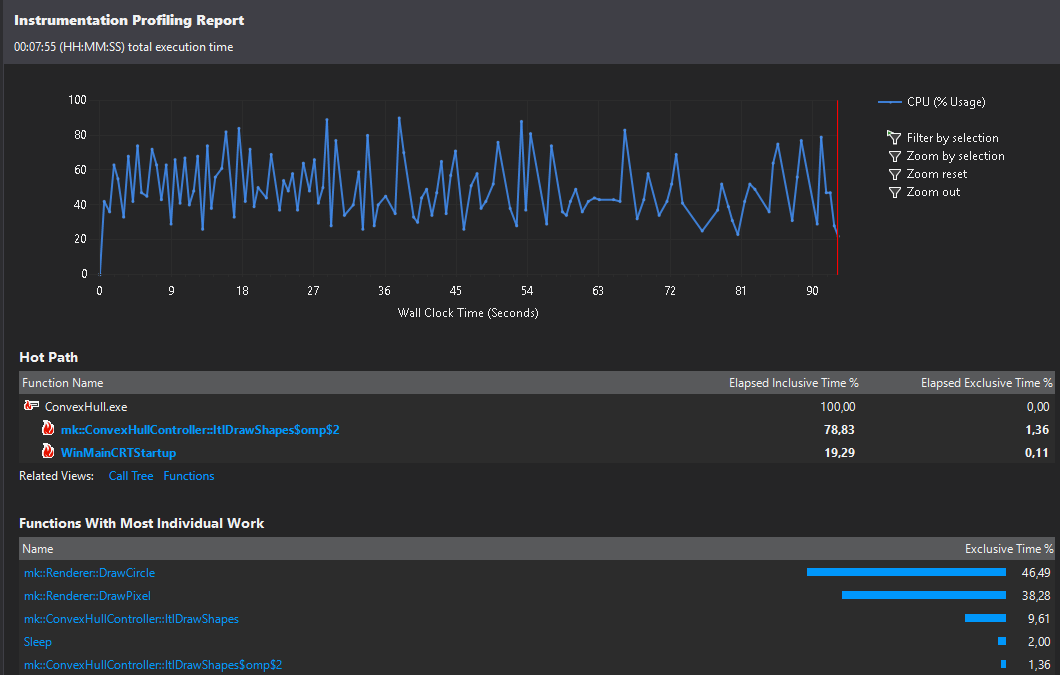
\includegraphics[scale = 0.275]{img/VisInstrumentationSummary.PNG}
\caption{Visual Studio Profiler CPU Instrumentation Summary}
\label{fig:VisualStudioProfilerInstrumentationSummary}
\end{figure}

\subsection{Concurrency}

The concurrency report follows the same structure again but is based on the thread contentions.

\begin{figure}[htbp]
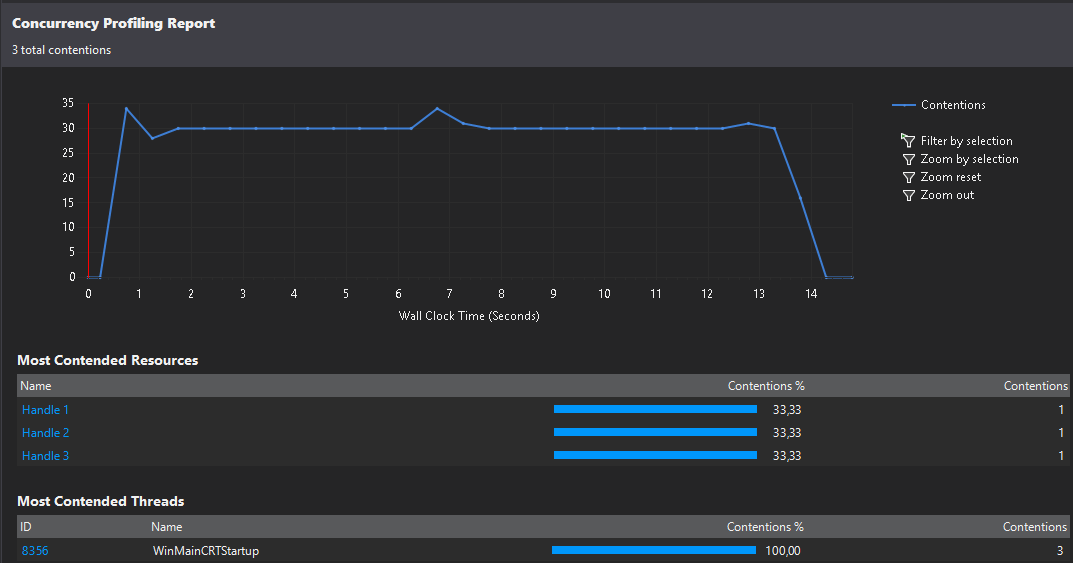
\includegraphics[scale = 0.275]{img/VisConcurrency.PNG}
\caption{Visual Studio Profiler CPU Concurrency Summary}
\label{fig:VisualStudioProfilerConcurrencySummary}
\end{figure}

\subsection{CPU/GPU Capture}

\begin{figure}[htbp]
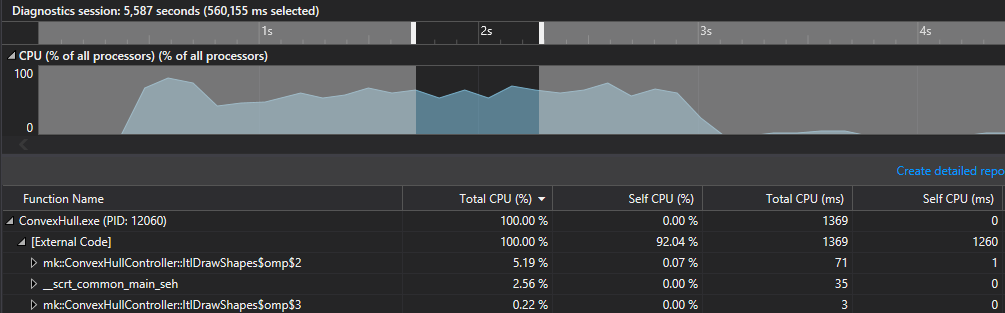
\includegraphics[scale = 0.30]{img/VisCPU.PNG}
\caption{Visual Studio Profiler CPU Capture}
\label{fig:VisualStudioProfilerCPUCapture}
\end{figure}

The simple CPU/GPU capture tools don not offer a detailed report but a simple CPU/GPU Usage and function breakdown.
Certain section of the execution time can also be selected for a function level breakdown of the selected time frame.

\subsection{Memory Capture}

The memory capture tools works a bit different because the snapshots have to be taken by the user during the profiling session.
A $"$Take Snapshot$"$ button will appear in the performance explorer window during the profiling session.

\begin{figure}[htbp]
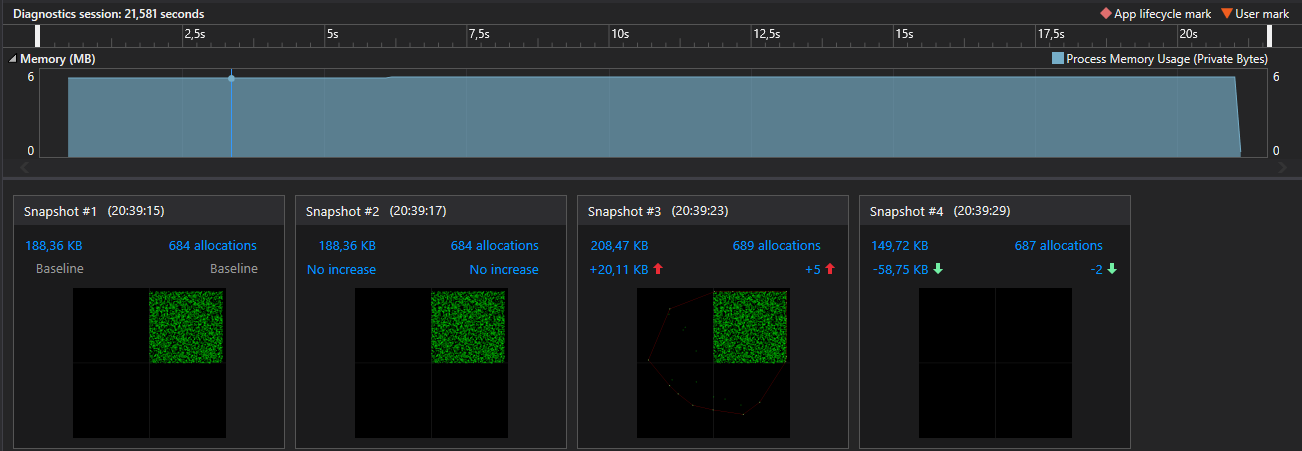
\includegraphics[scale = 0.23]{img/VisMemorySnapshots.PNG}
\caption{Visual Studio Profiler Memory Snapshots}
\label{fig:VisualStudioProfilerMemorySnapshots}
\end{figure}

The general memory usage is shown at the top with more detailed information for each snapshot.

\section{Unity Profiler}

The Unity Profiler is the profiler shipped with the Unity Engine, as of the current version (Unity v.5.2.3). It is found inside the Unity Editor tool under Window->Profiler. It can be run while testing the application in Unity and records performance Data later output as a timeline for analysis. It is frame accurate and can be used to see where spikes in eg. frametime occur during runtime and according to the Unity Documentation should be used to compare performance after code changes while providing minimal impact on performance.
Due to Unitys multiplatform compatibility some platforms (Android,iOS,Webplayer) require special steps in profiling which will not be discusses in this paper but can be found in the Unity documentation.


\subsection{Evaluation}

In accordance with the evaluation criteria provided in Section 3 the unity profiler was analysed. This analysis of the profilers capabilities yielded the following results.

\begin{table}[htbp]
\begin{tabular}{l|c}
Criteria & Availability \\ \hline \hline
CPU Sampling & \CheckedBox \\ \hline
Call Counts & \CheckedBox \\ 
Sampling Percentages & \CheckedBox \\ \hline
Time Measurement & \CheckedBox \\ \hline
Function Level Measurement* & \XBox \\ 
Line Level Measurement & \XBox \\ \hline
Memory Usage** & \CheckedBox \\ \hline
Memory Consumption & \CheckedBox \\
Heap Allocation & \XBox \\ 
Stack Allocation & \XBox \\ 
Memory Allocation/\\ Deallocation Time & \CheckedBox \\ \hline
Multithread support & \CheckedBox \\ \hline
\end{tabular}
\caption{Results Unity Profiler}
\label{tab:medfrequ}
\end{table}

*Time measurements are not provided for Functions of the actual code, but for calls to Unity functions that occur inside the code. Conclusions to the actual code can be drawn from these.\\
**Although there is not Heap and or Stack Allocation, Allocation for different relevant Objects is kept track of eg.Textures, Meshes, Materials.

The Unity Profiler is highly specialized to the fit the engines needs. In contrast to profilers for raw code it provides a lot more information that are relevant in the context of a game. All information is presented in a timeline and on a frame by frame basis. It contains information about CPU and GPU usage as audio sources, physics calls and network traffic. It does not provide a direct link to the program code, which requires the programmer to have a certain amount of insight into unity functions, since only those are represented in the profiler. Function calls implemented in will also show but most information needs to be deducted from the actual unity function calls.

\subsection{Using the Unity Profiler}

To start profiling with the Unity Profiler you need to open the project you want to profile and select the entry point for your game (eg. Main Menu) and open the profile which can be found inside the "Window" menu under "Profiler". The profiler window itself is composed of several sub-windows each representing a different timeline (eg. CPU Usage, GPU Usage, Memory Usage etc.). In the top of the profiling window are several options such as the record button, which enables you to record data while playing the game in the editor, the deep profiler, which allows you to profile all mono calls so you can debug your scripts and a Clear button. Furthermore it contains information about how much frames where recorded in total and which frame you are currently profiling, since all profiling is done in a frame by frame basis.  

\begin{figure}[htbp]
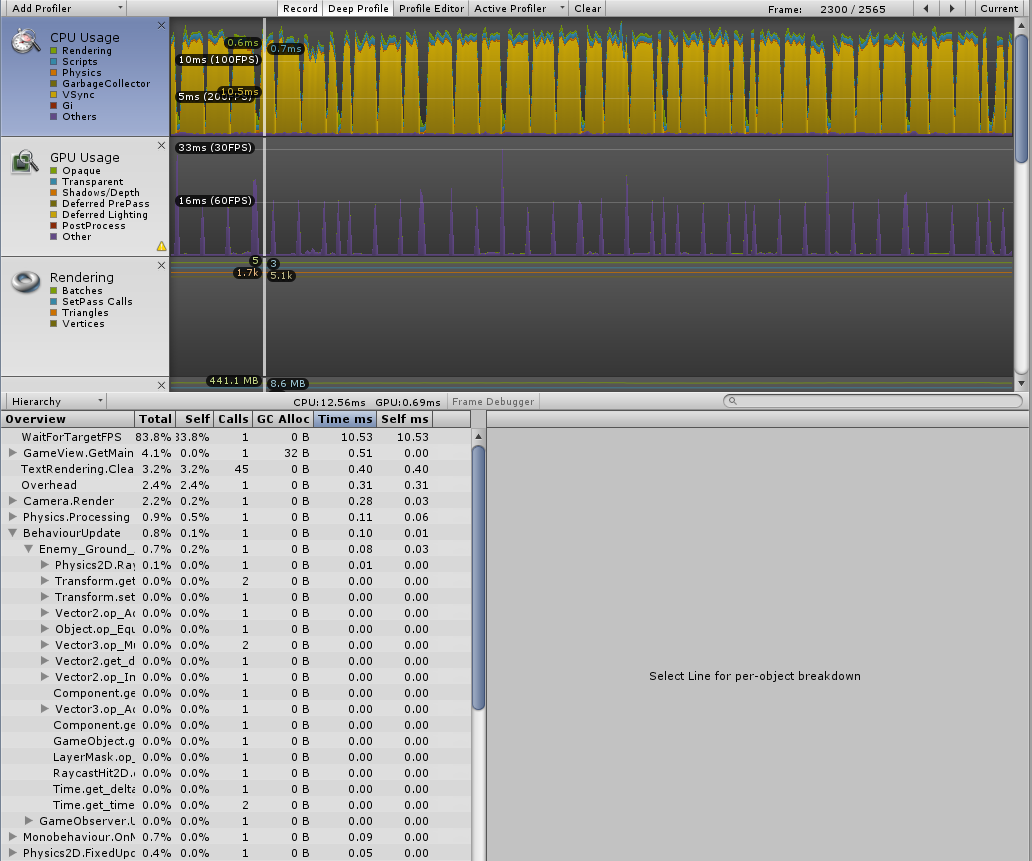
\includegraphics[scale = 0.29]{img/Unity_Profiler.PNG}
\caption{Unity Profiler Window}
\label{fig:UnityProfiler}
\end{figure}

The mouse cursor can be used to select the current frame inside the timeline and additional information is shown based on the context of the subprofiler. Additionally the bottom of the window shows more information about the currently selected sub-profiler shown in blue in \fref{fig:UnityProfiler}. \pagebreak

CPU Usage: \\ 
\\
In case of the CPU sub-profiler it shows either the Hierarchy of the calls as in \fref{fig:UnityProfiler} or the timeline. Either way the information is ordered by usage, highest usage first. Using this information the most impacting unity behaviours can be retrieved and further analysed. As seen in \fref{fig:UnityProfiler} the hierarchy is split up in parent and child calls. Parent Calls consist of high level Unity calls as for example the Behaviour.Update function. Inside these parents all children are shown and inside the children the individual Unity calls can be analysed such as Vector additions, transformation calls and physics calls.

Memory:

The memory sub-profiler, uses 2 different modes of displaying, the simple mode which shows high level memory usage and the detailed view, in context of this work the more interesting one. To get the detailed view of a frame the "Take Sample" button needs to be pressed. The result is a tabular representation of used memory, which is split up in different sections, with the Scene Memory part being the most relevant one, showing the memory usage of all objects inside the scene including their reference counts. This information can be used to profile memory restricted applications.\\

\begin{figure}[htbp]
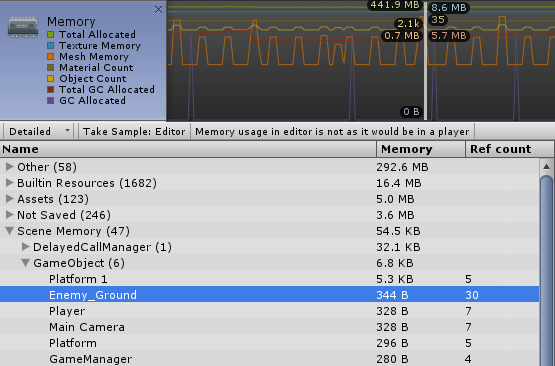
\includegraphics[scale = 0.53]{img/UnityProfilerMemory.PNG}
\caption{Unity Profiler Memory Area}
\label{fig:UnityProfilerMemory}
\end{figure}

Rendering:\\
\\
In the Rendering sub-profiler shows information such as Batches, Triangles, Vertices and SetPassCalls for the current frame. These are very similar to the rendering statistics window that can be enabled in the Editor during a running the game.

\begin{figure}[htbp]
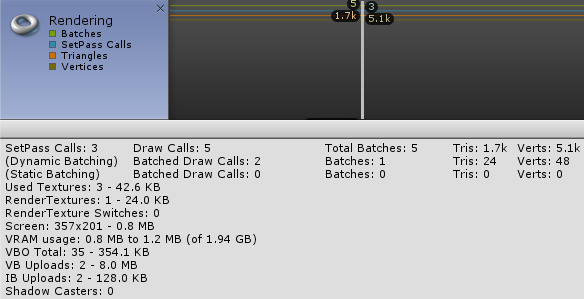
\includegraphics[scale = 0.53]{img/UnityProfilerRendering.PNG}
\caption{Unity Profiler Rendering Area}
\label{fig:UnityProfilerRendering}
\end{figure}

GPU:\\
\\
The GPU sub-profiler works like the CPU profiler and shows the number of DrawCalls and time spent inside each DrawCall. These are shown in a hierarchical way like in the CPU view. If the GPU profiler does not work for the current project it might be due to lack of the appropriate driver.

\begin{figure}[htbp]
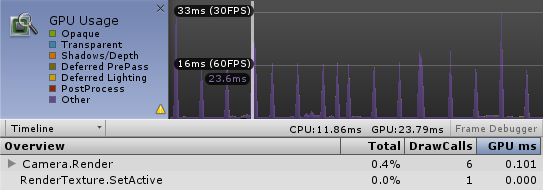
\includegraphics[scale = 0.53]{img/UnityProfilerGPU.PNG}
\caption{Unity Profiler GPU Area}
\label{fig:UnityProfilerGPU}
\end{figure}

Physics:\\
\\
Inside the Physics sub-profiler information about 2D and 3D physics can be found and is split up into five different kinds of Information.\\
Active Rigidbodies: These are currently moving physics objects inside of the inspected Frame\\
Sleeping Rigidbodies: Show the physics objects that are at rest and are not updated in the current frame.\\
Number of Contacts: Number of contacts of all colliders in the scene.\\
Static Colliders: Number of colliders not attached to rigidbodies.\\
Active Colliders: Number of colliders not attached to rigidbodies.\\

\begin{figure}[htbp]
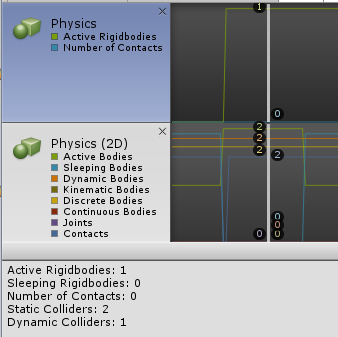
\includegraphics[scale = 0.53]{img/UnityProfilerPhysics.PNG}
\caption{Unity Profiler Physics Area}
\label{fig:UnityProfilerPhysics}
\end{figure}

\section{Unreal Engine Profiler}

The Unreal engine 4.9 offers its own profiler for CPU as well as GPU profiling. The profiler can be run in real time during the game for an immediate performance representation. Performance reports can also be saved and loaded later for a more in depth analysis.  Unreal also offers a simple fps breakdown of the workload. This breaks the performance down into multiple categories. 

\begin{figure}[htbp]
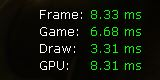
\includegraphics[scale = 0.8]{img/Unreal_Stat.jpg}
\caption{Unreal Stat Unit
https://docs.unrealengine.com
/latest/images/Engine/Performance/stat\_unit.jpg}
\label{fig:UnrealStat}
\end{figure}

First is the total frame time, Game represents the CPU game thread, Draw is the CPU render thread and GPU is the GPU time. This helps narrow down whether the CPU or the GPU should be profiled. The GPU is the bottleneck in the provided example. These frame rates can also be continuously captured over a period of time and combined into a graph.
\citep{unreal_performance_profiling}

\begin{figure}[htbp]
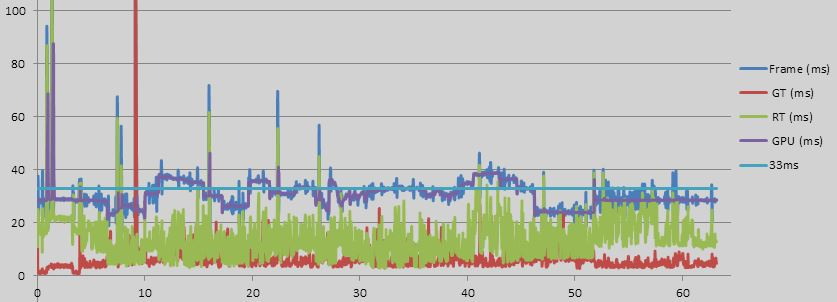
\includegraphics[scale = 0.3]{img/Unreal_FpsChart.jpg}
\caption{Unreal FPS Chart
https://docs.unrealengine.com
/latest/images/Engine/Performance/fpschart.jpg}
\label{fig:UnrealFPSChart}
\end{figure}


\section{Evaluation}
The Unreal profiler supports many of the evaluated features.

\begin{table}[htbp]
\begin{tabular}{p{5cm}|p{1cm}}
Criteria & Availability \\ \hline \hline
CPU Sampling & \CheckedBox \\ \hline
Call Counts & \CheckedBox \\ 
Sampling Percentages & \CheckedBox \\ \hline
Time Measurement & \CheckedBox \\ \hline
Function Level Measurement & \CheckedBox \\ 
Line Level Measurement & \XBox \\ \hline
Memory Usage & \CheckedBox \\ \hline
Memory Consumption & \CheckedBox \\
Heap Allocation & \CheckedBox \\ 
Stack Allocation & \XBox \\ 
Memory Allocation/Deallocation Time & \XBox \\ \hline
Multithread support & \CheckedBox \\ \hline
\end{tabular}
\caption{Results Unreal engine Profiler}
\label{tab:medfrequ}
\end{table}

The Unreal profiler provides most of the evaluated features.

\subsection{CPU Profiling}

The Unreal profiler is built into the editor of the Unreal engine. The profiler can be opened be selecting the $"$Window$"$ tab in the top menu of the editor then $"$Developer Tools$"$ and $"$Session Front end$"$. This opens the $"$Session Front end$"$ window where the profiler is located.

\begin{figure*}[!htbp]
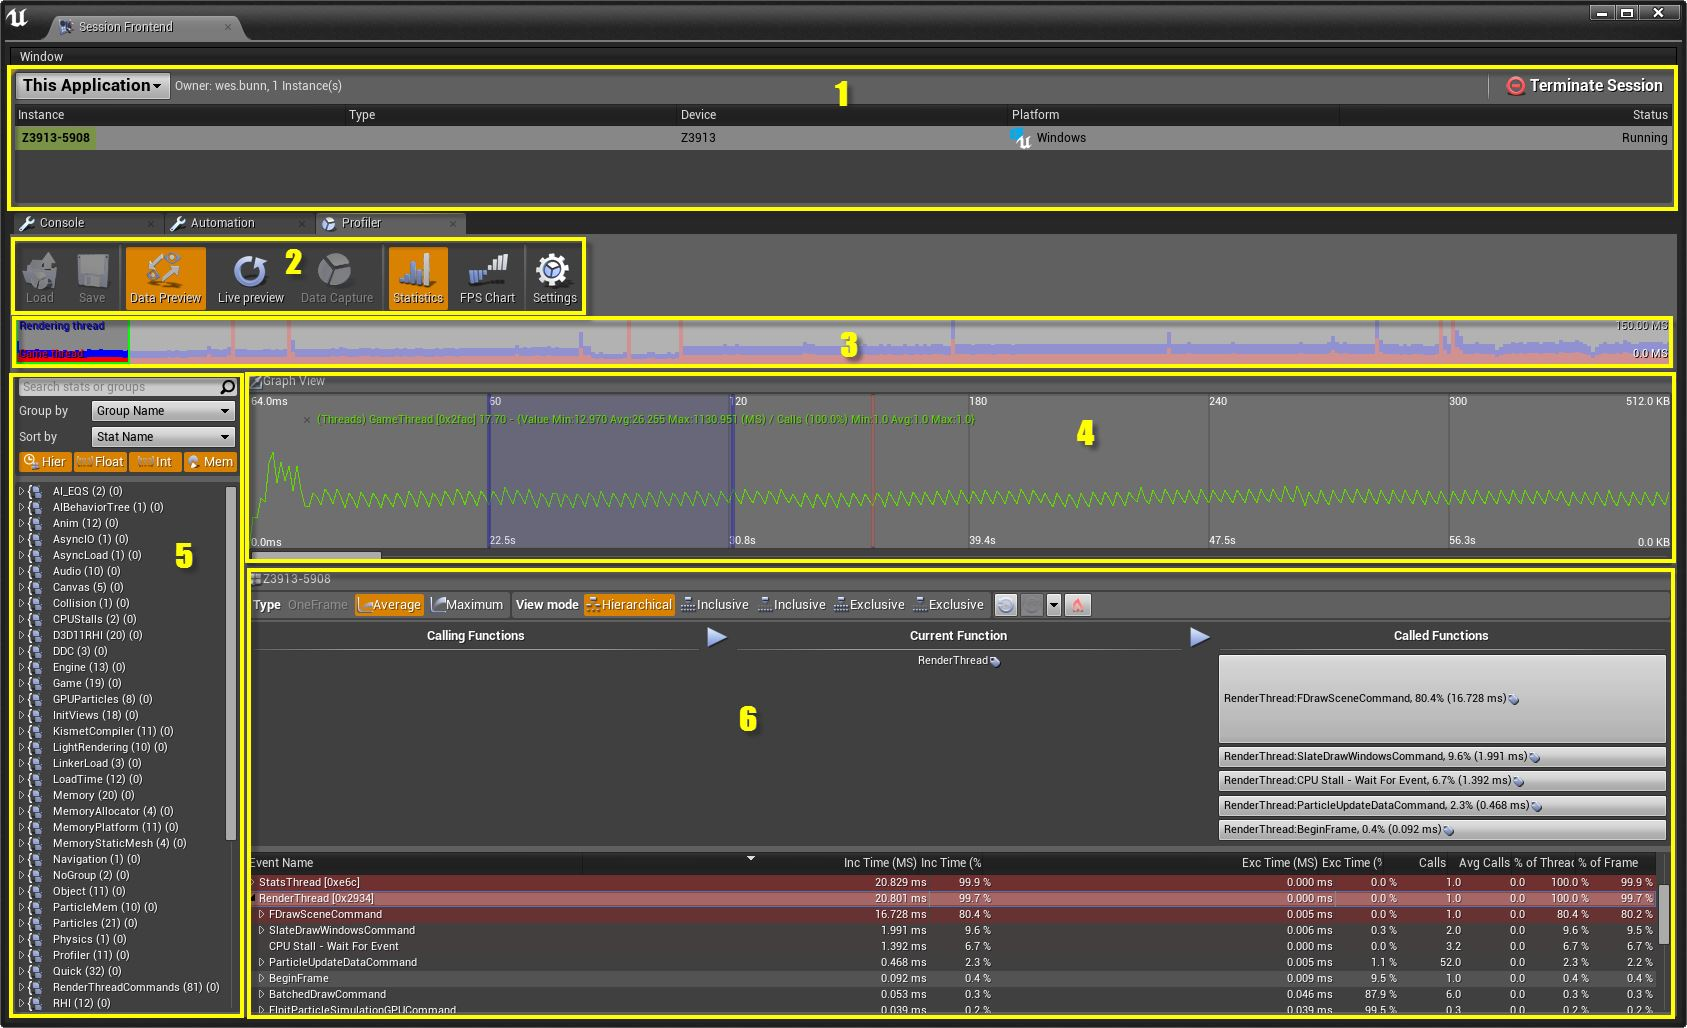
\includegraphics[scale = 0.35]{img/Unreal_SessionFrontend.jpg}
\caption{Unreal Session Frontend menu https://docs.unrealengine.com/latest/images/Engine/Performance/Profiler/ProfilierUI.jpg}
\label{fig:UnrealSessionFrontendMenu}
\end{figure*}

This is the complete $"$Session Front end$"$ window. It is separated into multiple sub-windows.

\subsubsection{1 Session Window}
The profiled session can be selected here and various session information is also displayed.
Below is various environment information such as the platform (Windows, PS4, ...).

\subsubsection{2 Main Toolbar}

\begin{figure}[htbp]
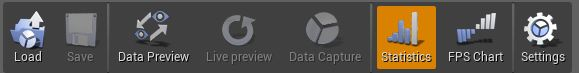
\includegraphics[scale = 0.5]{img/Unreal_MainToolbar.jpg}
\caption{Unreal Main Toolbar https://docs.unrealengine.com/latest/images/Engine/Performance/Profiler/Profiler\_MainToolbar.jpg}
\label{fig:UnrealMainToolbar}
\end{figure}

The main toolbar offers various profiling options. The profiling data can be loaded and saved. But the save option is currently not functional. $"$Data Preview$"$ starts a continuous capture of the profiling data. $"$Live Preview$"$ sets the currently displayed data automatically to the last captured frame. $"$Capture Data$"$ stores the captured profiling data which can be saved at the end. The last option is the $"$Fps Chart$"$. Note that this FPS chart is different from the one mentioned in at the beginning of the Unreal profiler. This creates a histogram of the FPS but does not include a breakdown of the FPS per pipeline stage.
\citep{unreal_profiler}

\begin{figure}[htbp]
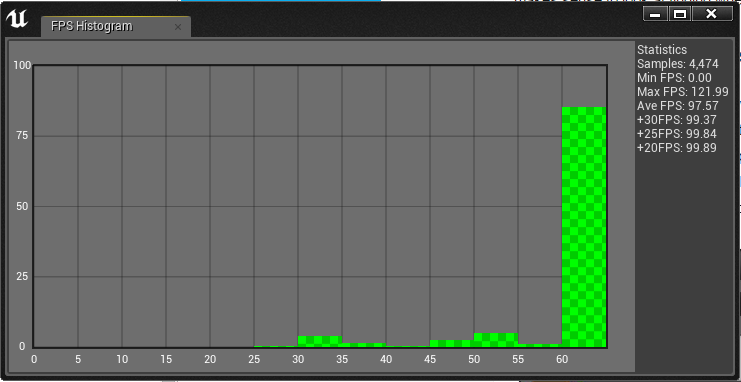
\includegraphics[scale = 0.39]{img/Unreal_FpsHistogram.PNG}
\caption{Unreal FPS Histogram}
\label{fig:UnrealFPSHistogram}
\end{figure}

This shows how many samples fall in a certain FPS bucket. Additional global information is also displayed on the right, such as the maximum, minimum as well as the sample percentages above certain FPS thresholds.

\subsubsection{3 Full Data Graph}
Below that is the full data graph. It provides a graphical overview of the entire profiling data. The bar chart shows the total time the render and game thread took. The highlighted section is used for the more detailed data graph below and can be moved in the full data graph.
\citep{unreal_profiler}

\subsubsection{4 Data Graph}
Bellow are the main data evaluation tools.

\subsubsection{5 Filter and Preset Window}

\begin{figure}[htbp]
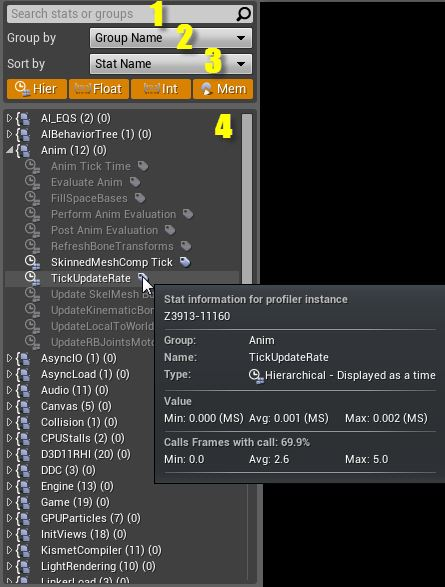
\includegraphics[scale = 0.39]{img/Unreal_FilterPresets.jpg}
\caption{Unreal Filter and Presets Window}
\label{fig:UnrealFilterPresets}
\end{figure}

To the left is the filter and presets window. The information that is to be displayed in the data graph is selected here. There is hierarchical structure view for the stats. These are sorted into integer, float and memory stats.
The stats can be filtered by their group, name and type (1, 2, 3). Every stat that is hovered in the stats window also displays the stat information such as the minimum, maximum and average values. The stats can be selected by clicking or dragging them to the data graph (4). Every selected stat is then tracked in the data graph.
\citep{unreal_profiler}

\subsubsection{6 Event Graph Window}

The event graph window is separated into two sub windows. The upper part is the data graph.

\begin{figure}[htbp]
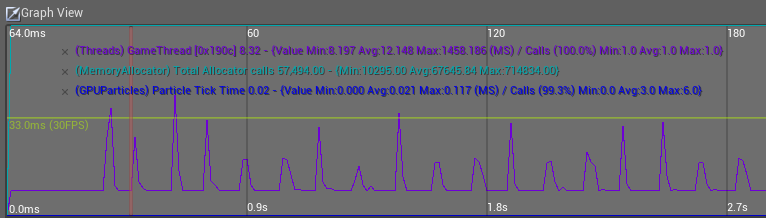
\includegraphics[scale = 0.39]{img/Unreal_DataGraph.PNG}
\caption{Unreal Data Graph}
\label{fig:UnrealDataGraph}
\end{figure}

Every selected stat has its information displayed as a text overlay. The time segment is the highlighted section on the full data graph window. The stats displayed for each stat are based on the entire profiling data and are not only based on the currently highlighted selection. The displayed information contains the current, minimum, maximum and average values. Hierarchical stats also show additional call information. They also show the percentage of frames with a call to the stat as well as the minimum, maximum and average calls to the stat. These values are again based on the entire profiling data.
\citep{unreal_profiler}

The lower part is the main event graph and the toolbar.

\begin{figure}[htbp]
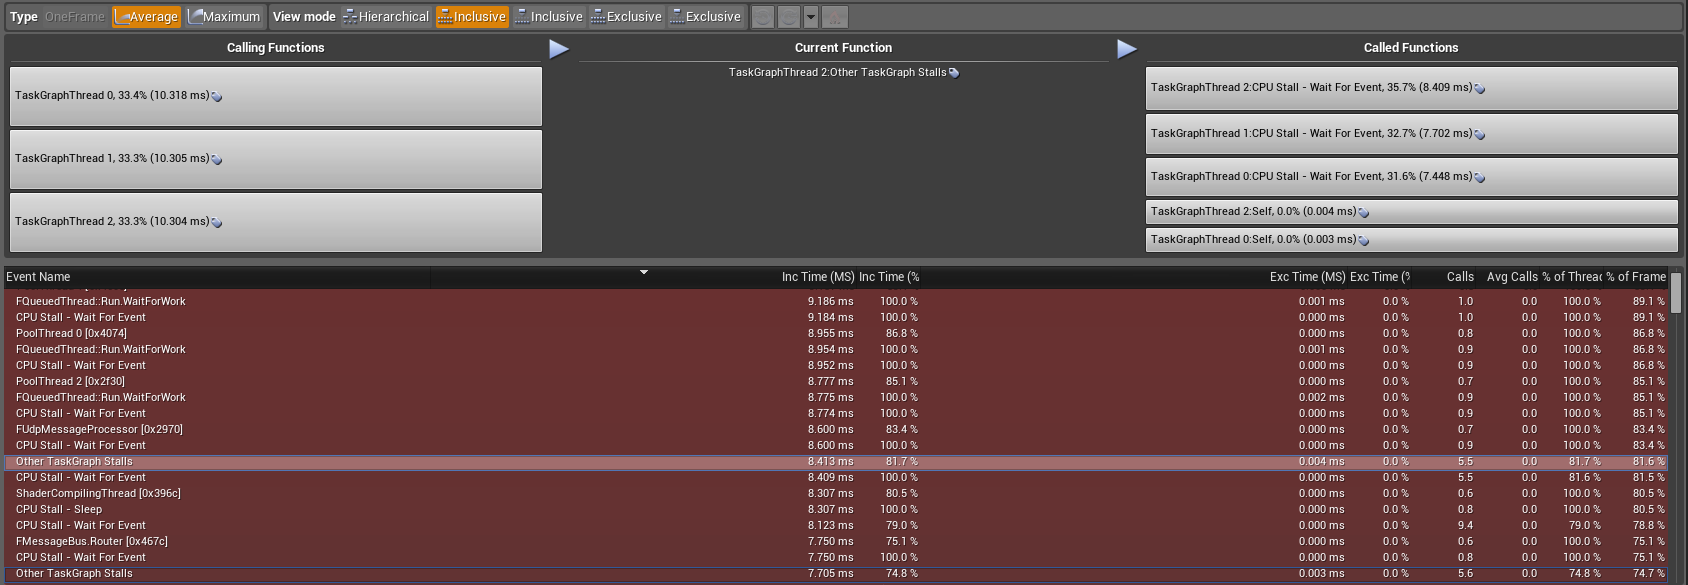
\includegraphics[scale = 0.18]{img/Unreal_EventGraph.PNG}
\caption{Unreal Event Graph}
\label{fig:UnrealEventGraph}
\end{figure}

The toolbar has multiple options to decide which information should be displayed. The information is based on the frames that have been selected in the data graph. The first section in the toolbar decides what type of information should be displayed

\begin{enumerate}
\item One Frame: Can be enabled if only one frame has been selected in the data graph. This only shows the information from a single frame.
\item Average: This can be enabled if multiple frames have been selected. This shows a per frame average graph.
\item Maximum: This can be enabled if multiple frames have been selected. This shows a per frame maximum graph.
\end{enumerate}
\citep{unreal_profiler}

The second section can be used to choose how the events are displayed and sorted in the main event graph.

\begin{enumerate}
\item Hierachical: This displays the events in a hierarchical tree view.
\item Inclusive: This displays the events as flat list sorted by the inclusive time.
\item Inclusive (different icon): This displays the events as flat list coalesced by the event name and sorted by the inclusive time.
\item Exclusive: This displays the events as flat list sorted by the exclusive time.
\item Exclusive (different icon): This displays the events as flat list coalesced by the event name and sorted by the exclusive time.
\end{enumerate}
\citep{unreal_profiler}

And the last section contains step back and step forward buttons and an option to display the hot path for the selected events.

The next part is are the function details. This shows the currently selected event and the functions or events that called the selected event. These are displayed as buttons and are scaled in relation to their performance impact. The windows is separated into three parts for the calling functions, the current function and the called functions respectively. The inclusive time in milliseconds and as a percentage are also shown for every function.
\citep{unreal_profiler}

The last part is the main event graph. This is a table with every event. The following information is displayed for every event. This information can also be shown in a separate window by hovering the event.

\begin{enumerate}
\item Event Name
\item Inclusive Time in milliseconds
\item Inclusive time as a percentage
\item Exclusive Time in milliseconds
\item Exclusive time as a percentage
\item The number of times the event has been called
\item The average number of times the event has been called
\item The inclusive time epercentage per thread.
\item The inclusive time epercentage per frame.
\end{enumerate}
\citep{unreal_profiler}

\subsection{GPU Profiling}

The GPU profiling is a bit more limited than the CPU profiler. The GPU profiler can be accessed by opening the unreal console and entering $"$profilegpu$"$. This opens a new window with the GPU data that has been captured up to this point. The data itself is based on GPU timestamps. It shows a timing breakdown of how long individual passes took. The timing breakdown is hierarchical and each pass can be broken down further. Sometimes down the draw calls.
\citep{unreal_gpu_profiling}

\begin{figure}[htbp]
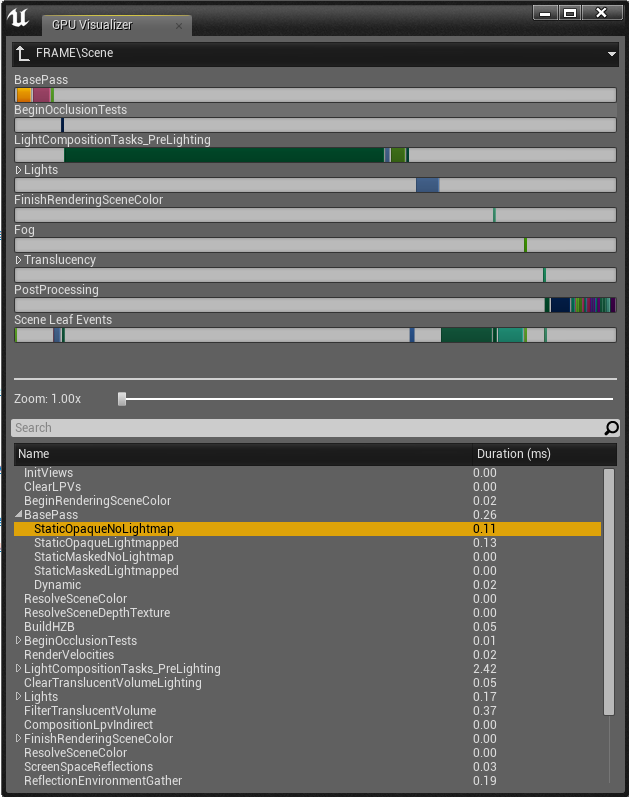
\includegraphics[scale = 0.45]{img/Unreal_GpuProfiler.PNG}
\caption{Unreal GPU Visualizer}
\label{fig:UnrealFPSChart}
\end{figure}

The profiler shows a graphical breakdown of the passes at the top with a multi level bar chart. Below is the hierarchical breakdown of the passes and their respective times. 

\section {Nvidia Nsight}

Nvidia Nsight is a debugger designed to debug programs running on Nvidia GPUs. In this work, we will focus on the NVIDIA Nsight Visual Studio 5.0 implementation, a additional software package for the Visual Studio IDE, providing all Nsight functionality inside Visual Studio. To use them an additional installation of the Nvidia Display Driver which supports Nsight is necessary. \cite{nvidia_nvidia_2015} lists the following drivers as compatible: Release 355.85 and Release 355 or newer. \\
Nvidia Nsight generally consists of three different functionalities. The CUDA Debugger, allows to debug applications using Compute Unified Device Architecture(CUDA), according to \cite{nvidia_nvidia_2015} it is able to inspect memory usage and perform memory checks in addition to normal debugging features such as breakpoints. Though the debugger only works on programs created with either the CUDA Runtime API or the CUDA Driver API.
The normal Graphics Debugger, can be utilised to debug a frame by each draw call, allowing you to inspect the shaders and pipeline. Furthermore this allows the profiling of graphics code together with the Analysis and Profiling tools. These show the workload of your system and shows API Calls (eg. OpenGl, CUDA) as well as memory management, draw calls and Events on the GPU and CPU.
Nsight can be configured in two different ways a pure client side version running the IDE and Nsight on the same machine, and a target and Host setup using an additional machine to debug code. This work will focus on the pure client side installation and addition information for the Target Host setup can be found on the Nvidia Nsight page.\citep {nvidia_nvidia_2015}

\begin{table}[htbp]
\begin{tabular}{p{5cm}|p{1cm}}
Criteria & Availability \\ \hline \hline
CPU Sampling & \CheckedBox \\ \hline
Call Counts & \XBox \\ 
Sampling Percentages & \XBox \\ \hline
Time Measurement & \XBox \\ \hline
Function Level Measurement & \XBox \\ 
Line Level Measurement & \XBox \\ \hline
Memory Usage & \CheckedBox \\ \hline
Memory Consumption & \CheckedBox \\
Heap Allocation & \CheckedBox\\ 
Stack Allocation & \XBox \\ 
Memory Allocation/Deallocation Time & \XBox \\\hline
Multithread support & \CheckedBox \\ \hline
\end{tabular}
\caption{Results Nsight Profiler}
\label{tab:medfrequ}
\end{table}

\subsection {Local Debugging}

To start using the local debugging feature of Nsight, the user first needs to check if the debugging machine fulfills all the requirements needed, including a supported Graphics card (the list can be found in the Nsight User Guide). After that the Nsight Monitor needs to be started, which is found under:

\textbackslash ProgramData\textbackslash Microsoft\textbackslash Windows\textbackslash Start Menu\textbackslash Programs\textbackslash NVIDIA Corporation\textbackslash Nsight Visual Studio Edition 5.0\\

After starting Nsight it will appear in the taskbar and can be opened with a double click on the icon. This needs to be started in order to use Nsight, and will automatically be started if Nsight is used inside the Visual Studio IDE.\\

\subsubsection {The Frame Debugger}

Using the Graphics Debugger enables the user to utilise the Frame debugger to debug frames in realtime. Rendering calls can be examined as well as the the pipeline state, it provides an visualisation to help debug as well. Captures Frames can be saved and analysed offline as well as profiled.
It additionally provides a Heads up Display which overlays over the debugged application and can be customized with additional graphs. It also enables four additional modes:
\begin{enumerate}
\item Depth Complexity View: This shows how much geometry is overdrawn every drawcall.
\item 2X2 textures: Provides insight into the application in term of it being texture bound
\item Null Scissor Rectangle: Provides insight into the application in term of it being pixel bound 
\item Minimum Grometry: Shows whether the application is CPU or GPU bound by drawing only the first triangle of each draw call. Rising framerates indicate a GPU bound application, while no change indicates a CPU bound application.
\end{enumerate}

\begin{figure}[htbp]
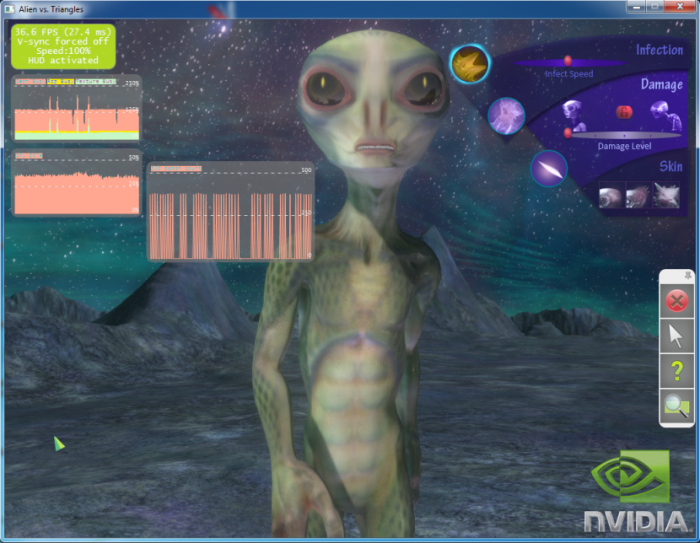
\includegraphics[scale = 0.42]{img/Nsight_HUd.png}
\caption{Nsight Frame Debugger HUD http://docs.nvidia.com/nsight-visual-studio-edition/5.0/Content/Images/HUD.Main.RunMode\_700x543.png}
\label{fig:Nsight_Hud}
\end{figure}

You can enter the Debugger directly form the HUD by either pressing CTRL+Z or in the Visual Studio Menu under Nsight, by pressing the Pause and Capture Frame button. Doing this enables you to use a set of options, like rendering the Depth buffer or the stencil buffer instead of the image or displaying the Scene in Wireframe mode.\\
When Debugging a Frame there are various tools available to the user. One of them are Performance Markers which can be set in four different ways, via the NVTX tool extension, OpenGL command such as KHR\_debug group, glPushDebugGroup and glPopDebugGroup, Direct3D 11.1 Commands like ID3DUserDefinedAnnotation and the Direct3D 9 commands D3DPERF\_BeginEvent and D3DPERF\_EndEvent. These can be used to mark a section of events for time measurement. Time spent in Sections between the markers will be measured and can be analyzed in either the Scrubber or the HUD. The Sections will be highlighted in the defined marker color in graphical representations respectively.

\begin{figure}[htbp]
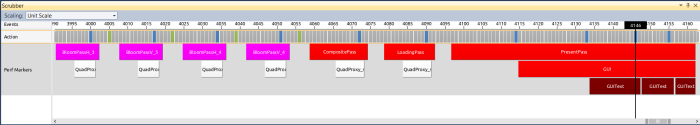
\includegraphics[scale = 0.42]{img/NSight_Scrubber.png}
\caption{Nsight Scrubber http://docs.nvidia.com/nsight-visual-studio-edition/5.0/Content/Images/Graphics\_Perf\_Markers.001\_700x125.png}
\label{fig:Nsight_Scrubber}
\end{figure}

Events can also be inspected individually in the Events Page of the Frame Debugger, nested events will also be displayed in dropdown menus. The Event lost shows all API Calls and highlights performance marked Segments in their respective color.
An additional Page of information is the API Statistics Page which provides information on the API Calls as well as the amount of times they have been called. To open this windows the user needs to access the Nsight menu in visual studio, select windows and then the API Statistics window.

\begin{figure}[htbp]
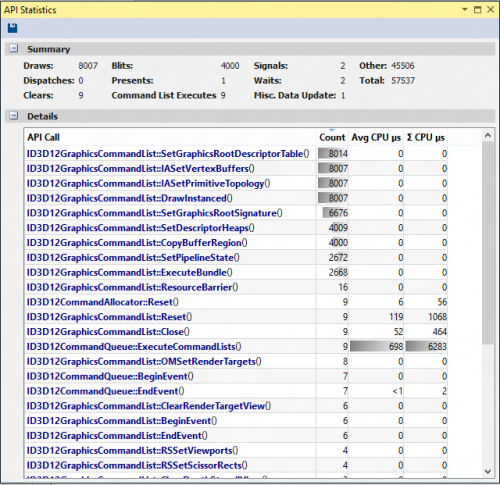
\includegraphics[scale = 0.42]{img/Nsight_API_statistics.png}
\caption{Nsight API Statistics http://docs.nvidia.com/nsight-visual-studio-edition/5.0/Content/Images/graphics\_d3d12\_api\_statistics.002\_500x485.png}
\label{fig:Nsight_API_Statistics}
\end{figure}

Additional information about the current Frame includes Heap information, which shows all created heaps with their respective resources and resource Types.
Some additional features are Graphics API specific and can be read up on in the Nsight User Guide on Nvidias page.

\subsubsection {Analysis Tools}

The analysis Tools allows the user to run the program and attach a trace to it which at then end of recording or at the end of the programs execution creates a detailed report showing all activity during the program including events from other programs and a lot more depending on the selected settings.

To start using the Analysis Tools the user needs to click on the Nsight menu in Visual Studio 2015 and select the Start Performance Analysis option. Which opens the Activity Document. Inside this Form the user can select what and how he wants to profile his application.\\
First part is the Application Settings which contains information like the debug mode (local or remote) and where the application an its working directory are located.\\
The Triggers and Actions tab governs when the information gathering is started and stopped, this can be set to automatic(Program start, and End) or to manual respectively.\\
The Activity Type sets the kind of analysis that gets performed. The most important here are Trace Application, which traces data from a single target application and Trace Process Tree, which also includes all child processes in the trace.\\
The Trace and Profiler Settings contain the data you want to trace and is split in System,Tools Extension, CUDA, OpenCL, DirectX and OpenGl. Each of them also contain subtraces which can be switched on and off individually but for the sake of this work the most important are the following:
\begin{enumerate}
\item System: Traces CPU usage
\item Tools Extension: In case Performance Markers ares used these are also taken into consideration during the tracing process
\item DirectX: Provides an API Trace as well as GPU information
\item OpenGL: Provides an API Trace as well as GPU information
\end{enumerate}

\begin{figure}[htbp]
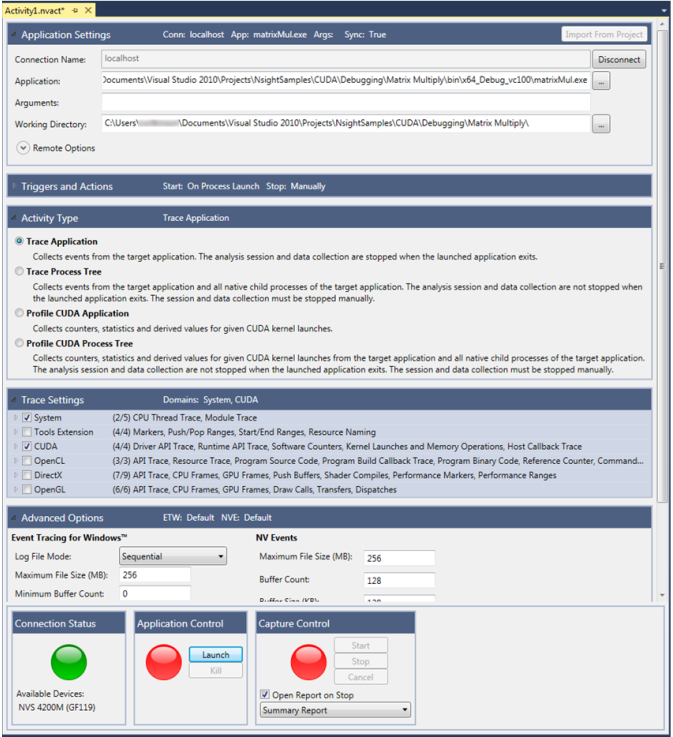
\includegraphics[scale = 0.42]{img/NSight_Application_Document.png}
\caption{Nsight Activity Document}
\label{fig:Nsight_Activtiy_Page}
\end{figure}

Advanced Options typically do not need and should not to be adjusted.\\
The last Section is the Launch an capture control which is split into three parts. The connection status, which shows whether Nsight is connected to a Nvidia device, the Application control which lets the user start and terminate the application and the capture control, that is used to start and stop the capture process.

\section{Analyze the collected Data. Step by Step}

\begin{enumerate}
    \item Start the Nvidia Nsight Monitor
    \item Start Visual Studio
    \item Select the project you want to analyze and create a build of the project
    \item Select $"$Start Performance Analysis$"$ form the Nsight menu
    \item Select the data you want to trace see section 7.1.2 
    \item Click the Launch button to start the application
    \item If manual capture is selected click the start button under the capture section
    \item Click the Kill Button to stop the application and the Capture
\end{enumerate}

These steps lead to the automatic opening of the NVReport.

\begin{figure}[htbp]
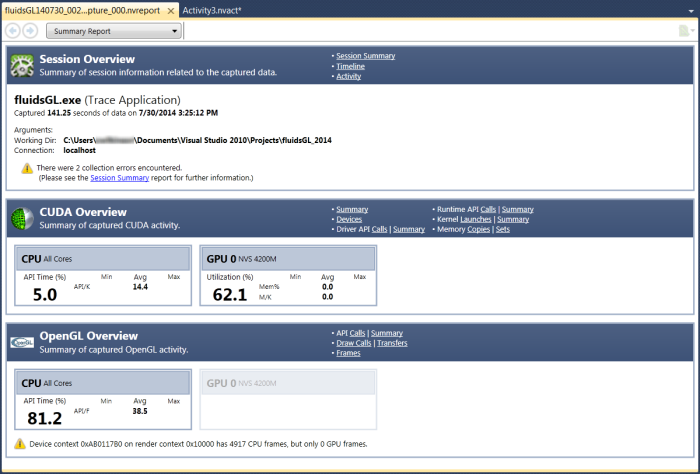
\includegraphics[scale = 0.4]{img/NSight_NVReport1.png}
\caption{Nsight Summary Report
http://docs.nvidia.com/nsight-visual-studio-edition/5.0/Content/Images/
Analysis\_SummaryReport.003\_700x474.png}
\label{fig:Nsight_NVReport1}
\end{figure}

\fref{fig:Nsight_NVReport1} shows the $"$Summary Report$"$. The top left corner shows a dropdown menu which can be opened to see each segment of the report that corresponds with your selected trace targets. Basic information is always displayed under the $"$Summary Report$"$ tab.

\begin{figure}[htbp]
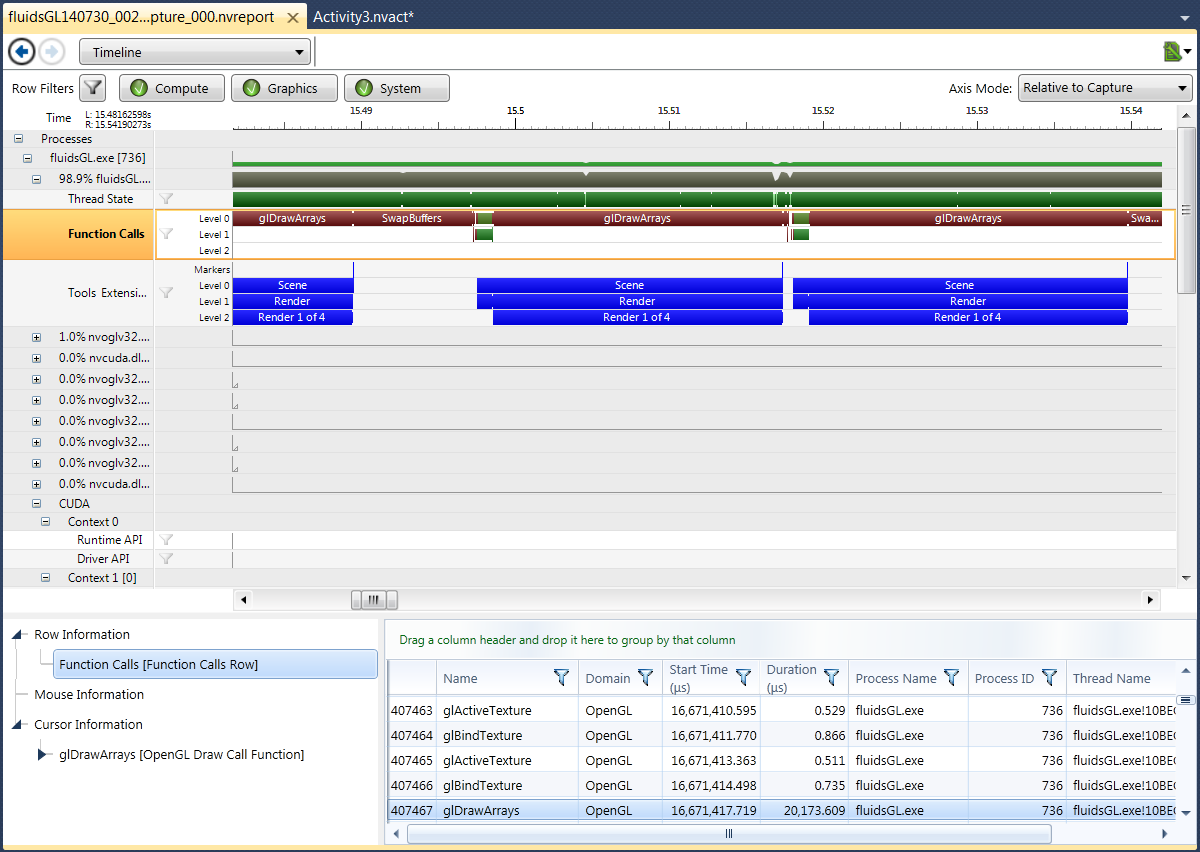
\includegraphics[scale = 0.3]{img/NSight_NVReport2.png}
\caption{Nsight Timeline
http://docs.nvidia.com/nsight-visual-studio-edition/5.0/Content/Images/Analysis\_TimelinePage.003.png}
\label{fig:Nsight_NVReport2}
\end{figure}

\fref{fig:Nsight_NVReport2} shows the timeline. This Tab will also always be present in every report and enables in depth analysis of the System during the captured timeframe. These include API calls, CPU usage by other programs during the runtime as well as GPU usage. Using the Timeframe information such as how well the GPU is fed can be deduced to further optimize the Application. For Example if the GPU is idle a lot of the time maybe it is due to to much communication between GPU and CPU and calls need to batched.

\section{Additional Features}

\subsection{Frame Serializer}

During the use of the Frame Debugger, a frame can be captured and serialized. 
\begin{figure}[htbp]

\includegraphics[scale = 1]{img/NSight_Save.png}
\caption{Nsight Frame Debugger Overlay save Button}
\label{fig:Nsight_Save}
\end{figure}

The Button displayed in \fref{fig:Nsight_Save} will be prominent in the top right of the screen during debugging and enables the serialization oft the current frame. This data can then be sent to other users of Nsight to analyzed there. This enables the possibility to share bugs with other members of the development team as well as Nvidia for optimizing their drivers.

\section{AMD CodeXL}

AMD offers its own profiler and performance analyser CodeXL. This a a new program that succeeds the previous AMD CodeAnalyst as AMDs profiling and debugging tool. This profiler was specially built to profile AMDs product line of CPUs, GPUs and APUs. CodeXL is available as a standalone application for Windows and Linus as well as a Visual Studio extension. A more detailed tutorial for CodeXL is omitted a this point as the authors do not have access to the AMD products necessary to properly familiarize themselves with the program.
\citep{amd_codexl}

\section{Evaluation}

\begin{table}[htbp]
\begin{tabular}{p{5cm}|p{1cm}}
Criteria & Availability \\ \hline \hline
CPU Sampling & \CheckedBox \\ \hline
Call Counts & \XBox \\ 
Sampling Percentages & \CheckedBox \\ \hline
Time Measurement & \XBox \\ \hline
Function Level Measurement & \CheckedBox \\ 
Line Level Measurement & \XBox \\ \hline
Memory Usage & \XBox \\ \hline
Memory Consumption & \XBox \\
Heap Allocation & \XBox\\ 
Stack Allocation & \XBox \\ 
Memory Allocation/Deallocation Time & \XBox \\ \hline
Multithread support & \CheckedBox \\ \hline
\end{tabular}
\caption{Results AMD CodeXL}
\label{tab:medfrequ}
\end{table}

The CodeXL CPU profiler relies heavily on CPU Sampling and omits memory tracking and time measurements.

\section{CPU Profiling}

The CPU profiler allows for time or instruction based sampling. The sample counts and relative sample measurements are then collected and displayed on a per function level. This allows for relative performance analysis. The sampling is realised through hardware level performance counters and should as such have a minimal performance impact and offer accurate readings.
\citep{amd_codexl_details}

\begin{figure}[htbp]
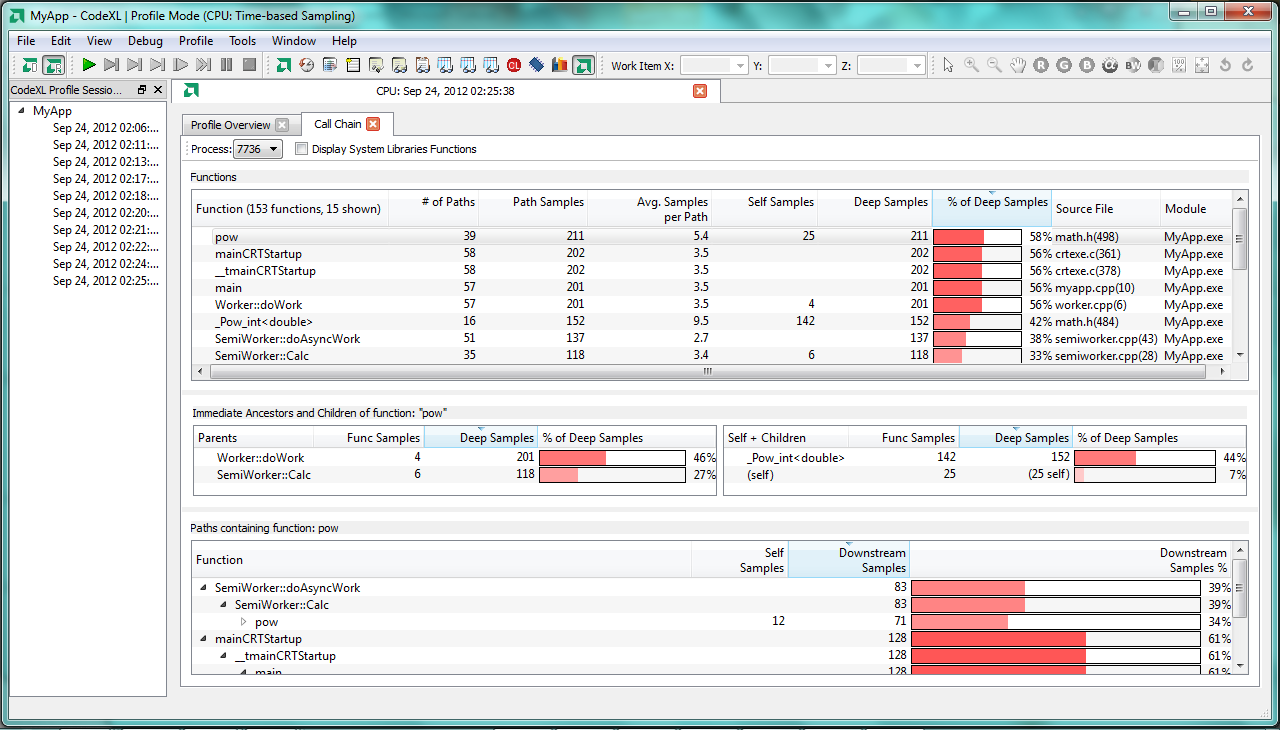
\includegraphics[scale = 0.23]{img/AMD_Sampling.png}
\caption{CodeXL Time-based Sampling 
http://amd-dev.wpengine.netdna-cdn.com/wordpress/media/2012/10/2\_TBP.png}
\label{fig:AMD_Sampling}
\end{figure}

CodeXL also offers call chain relationship analysis. This shows the functions in relation to their caller and callee. All CPU profiling features also work with with multiple threads. CodeXL also measures various CPU metrics such as CPU frequency, and CPU core thermal data.
\citep{amd_codexl}

\section{GPU Profiling}
CodeXL offers real time API level debugging for OpenCL and OpenGL which shows the API function calls and which code paths led to them. Shader code can also be debugged by exporting the compiled file during runtiume and then loading it into CodeXL for debugging. Performance data is also collected through GPU counters, application trace, kernel occupancy and hotspot analysis. The data is gathered during run time and can then be evaluated. It also offers various GPU metrics such as the power consumption of discrete GPU components as well as thermal data and the GPU frequency. The GPU memory access characteristics and the actual execution time of the kernels are also tracked.
\citep{amd_codexl, amd_codexl_details}



%-- figure over both columns

%\begin{figure*}[!hbp]
%
\includegraphics[scale = 0.5]{img/test3.png}
%\caption{ caption \protect with citation %\cite{smeets_throwing_2002}}
%\label{fig:test1}
%\end{figure*}

% Bibliography



% Option 1: Bibliography generation with BibTeX:
% Add all refernces to the *.bib file (here Literatur.bib). Then run LaTeX, BibTeX, and again twice LaTeX.
% Use \cite{kop05} within the text for a citation.
% - GEMRAN ----------
%\bibliographystyle{apalike-url-de} %ermöglicht longnamesfirst Option. Bei erster Erwähnung werden alle Autoren gennannt in der Folge et al. verwenden wir aber nicht
% - END GERMAN-------
%% -ENGLISH---------

%\bibliographystyle{apalike-url}
%%% -END ENGLISH------
%\bibliography{Bibliography-Profiling}
% Option 2: Bibliography generation without BibTeX:
%\begin{thebibliography}{99}
%\bibitem[kop05]{kop05}
%H.~Kopka, {\em LaTeX, Band 1: Einf"uhrung}, Pearson Studium, M"unchen, 3.~Auflage, 2005.
%\bibitem[knu98]{knu98}
%F.~Mittelbach, M.~Goossens, J.~Braams, D.~Carlisle, and Ch. Rowley, {\em The LaTeX Companion}, 
%Addison-Wesley, 2nd edition, 2004.
%\end{thebibliography}

%\end{document}